%!TEX program = xelatex
%Template created by: Maciej Byczko
\documentclass[a4paper,12pt]{extarticle}  %typ dokumentu

\usepackage{geometry} %poprawienie marginesów
\usepackage{polski} %polskie znaki
\usepackage{graphicx} %grafiki
\usepackage{float} %poprawienie pozycji
\usepackage{fancyhdr} % header i footer
\usepackage{listings}
\usepackage{xcolor}
\graphicspath{{pictures/}}
\geometry{margin=0.7in}
\pagestyle{fancy}
\cfoot{Strona \thepage}
\rhead{Strona \thepage}
\lhead{\typdoc}
\setlength{\headheight}{15pt}

\title{\tytul \\ \small{\opis}}
\author{\tworcy}
\date{\data}

%-----------------------SEKCJA DANYCH----------------------------------
\def\tytul{Analizator parametrów sieci - EMA-90N} %<<< tytuł ćwiczenia
\def\nrcw{laboratoria 18} %<<< numer ćwiczenia
\def\data{\today} %<< data wykonania
\def\prowadzacy{Dr inż. Dominik Żelazny} %<<<prowadzący
\def\nrgrupy{D} %<<<numer grupy
\def\tworcy{Baraniecki Karol\\Byczko Maciej} %<<< autorzy
\def\zajinfo{PT 16:30 TP} %<<< informacje dotyczące zajęć
\def\typdoc{Sprawozdanie} %<<< typ dokumentu tj Sprawozdanie, zadania itp. {Matematyka dyskretna/Sprawozdanie z Miernictwa}
\def\opis{} %<<< opis który będzie umieszczony pod tytułem w Maketitle
%----------------------------------------------------------------------

\definecolor{backcolour}{rgb}{0.95,0.95,0.92}
\definecolor{AO}{rgb}{0,0.5,0}
\definecolor{ZeroBlue}{rgb}{0,0.28,0.73}
\definecolor{DarkRed}{rgb}{0.85,0.16,0.16}


\lstset{
basicstyle=\footnotesize,
breaklines=true,
language=Python,
numbers=left,
tabsize=2,
numberstyle=\tiny,
backgroundcolor=\color{backcolour},
breakatwhitespace=false,
showspaces=false,                
showstringspaces=false,
showtabs=false,
commentstyle=\color{gray},
keywordstyle=\color{ZeroBlue},
keepspaces=true,
% keywordstyle={[2]\color{DarkRed}},
% keywordstyle={[3]\color{ZeroBlue}},
}

\begin{document}
%-------------------------------------TABELA-DANYCH--------------------------------------------------
\begin{table}[H]
	\centering
	\resizebox{\textwidth}{!}{
		\begin{tabular}{|c|c|c|}\hline
			\begin{tabular}[c]{@{}c@{}}                     \tworcy     \end{tabular} &
			\begin{tabular}[c]{@{}c@{}}Prowadzący:\\        \prowadzacy \end{tabular} &
			\begin{tabular}[c]{@{}c@{}}Numer ćwiczenia\\    \nrcw       \end{tabular}          \\ \hline
			\begin{tabular}[c]{@{}c@{}}                     \zajinfo    \end{tabular} &
			\begin{tabular}[c]{@{}c@{}}Temat ćwiczenia:\\   \tytul      \end{tabular} & Ocena: \\ \hline
			\begin{tabular}[c]{@{}c@{}}Grupa:\\          \nrgrupy    \end{tabular} &
			\begin{tabular}[c]{@{}c@{}}Data wykonania:\\    \data       \end{tabular} &        \\ \hline
		\end{tabular}}
\end{table}
%----------------------------------------------------------------------------------------------------
\section{Zadania do opracowania}
\subsection{Sieć elektryczna}
\begin{itemize}
	\item napięcie - różnica potencjałów elektrycznych między dwoma punktami obwodu elektrycznego lub pola elektrycznego.
	\item prąd - uporządkowany ruch ładunków elektrycznych
	\item moc czynna - część mocy, którą odbiornik pobiera ze źródła i zamienia na pracę lub ciepło.
	\item moc bierna - wielkość opisująca pulsowanie energii elektrycznej między elementami obwodu elektrycznego.
	\item cos($\phi$) - Współczynnik mocy, stosunek mocy czynnej do mocy pozornej, czyli stosunek mocy użytecznej do iloczynu napięcia i prądu. 
	\item harmoniczna prądu
\end{itemize}
\subsection{Ethernet}
\begin{itemize}
	\item IP (Internet Protocol) - protokół komunikacyjny warstwy sieciowej modelu OSI (warstwy internetu w modelu TCP/IP).
	\item Maska - liczba służąca do wyodrębnienia w adresie IP części będącej adresem podsieci i części, która jest adresem hosta w tej podsieci. 
	\item Brama domyślna - router, do którego komputery sieci lokalnej mają wysyłać pakiety o ile nie powinny być one kierowane w sieć lokalną lub do innych, znanych im routerów.
	\item DHCP (Dynamic Host Configuration Protocol) - protokół komunikacyjny umożliwiający hostom uzyskanie od serwera danych konfiguracyjnych, np. adresu IP hosta, adresu IP bramy sieciowej, adresu serwera DNS, maski podsieci.
\end{itemize}
\subsection{Protokół modbus TCP/IP}
Modbus to popularny protokół komunikacyjny w którym komunikacja między urządzeniami realizowana jest w architekturze master-slave/client-server. 
Jest to protokół typu otwartego, co oznacza iż wszystkie niezbędne informacje do jego implementacji są ogólnodostępne.
\subsection{Bezpieczeństwo pracy z prądem}

\section{Zadania do wykonania}
\subsection{Połączyć urządzenie EMA-90N z komputerem za pomocą komunikacji Ethernet}
Ten podpunkt udało się wykonać bez większych problemów, urządzenie ma publiczne IP dzięki czemu można się do niego połączyć z dowolnej sieci.
\subsection{Uruchomienie aplikacji demonstracyjnej,połączenie się z urządzaniem odczytując napięcie i prąd na L1}
Chwilę zajęło aby ogarnąć interfejs lecz okazał się on prosty w użyciu i bardzo szybko odczytaliśmy wartości.

	
	\begin{figure}[H]
		\centering
		\resizebox*{\textwidth}{!}{
			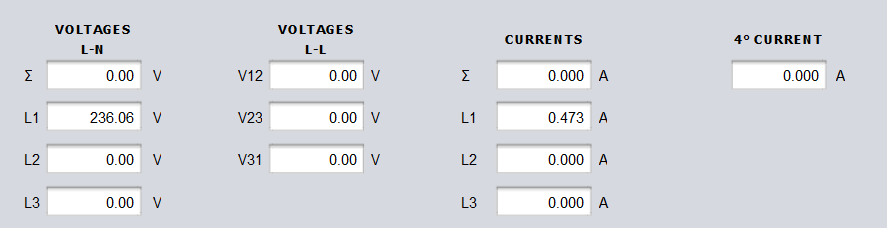
\includegraphics{readFromApp.png}
			}
		\end{figure}

		\begin{figure}[H]
		   \centering
		   \resizebox*{0.5\textwidth}{!}{
			  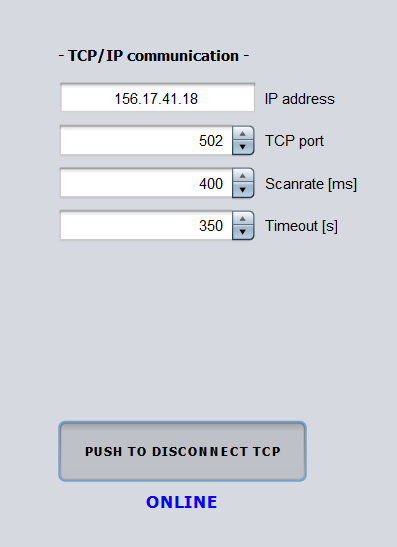
\includegraphics{connection.png}
		   }
		\end{figure}

Wada tej aplikacji jest taka że bardzo rzadko się odświeżają się wartości (raz na ~5 sekund)
\subsection{Napisanie aplikacji w Pythonie, połączenie sie z urządzenie i odczytanie napięcia i natężenia prądu na L1 poprzez protokół modbus}
Znaleźliśmy problem że do urządzenia nie może być podłączone kilka programów lecz oprócz tego bezproblemowo napisaliśmy kod, który odczytuje i wyświetla wartości w czasie rzeczywistym.
% \lstinputlisting{zaj2.py}
\begin{figure}[H]
   \centering
   \resizebox*{\textwidth}{!}{
	  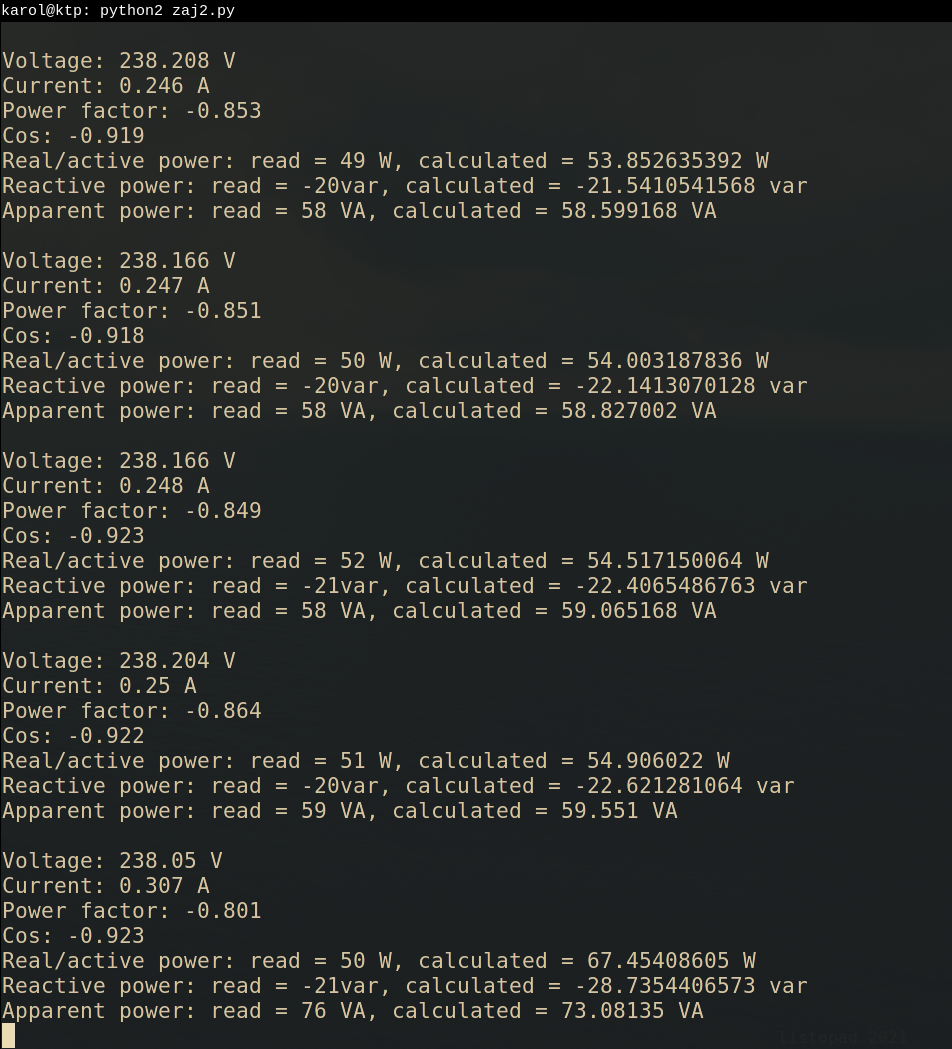
\includegraphics{zaj2.png}
   }
\end{figure}
Za pomocą aplikacji porównaliśmy odczyty urządzenia z obliczeniami i zauważyliśmy że któryś z parametrów ma znaczną niepewność pomiarową
\cleardoublepage
\section{Wnioski}
\subsection{Porównanie wyników}
\begin{center}
	Pomiary lampy
\end{center}
\begin{minipage}[c]{0.49\linewidth}
	\begin{figure}[H]
	   \centering
	   \resizebox*{\textwidth}{!}{
		  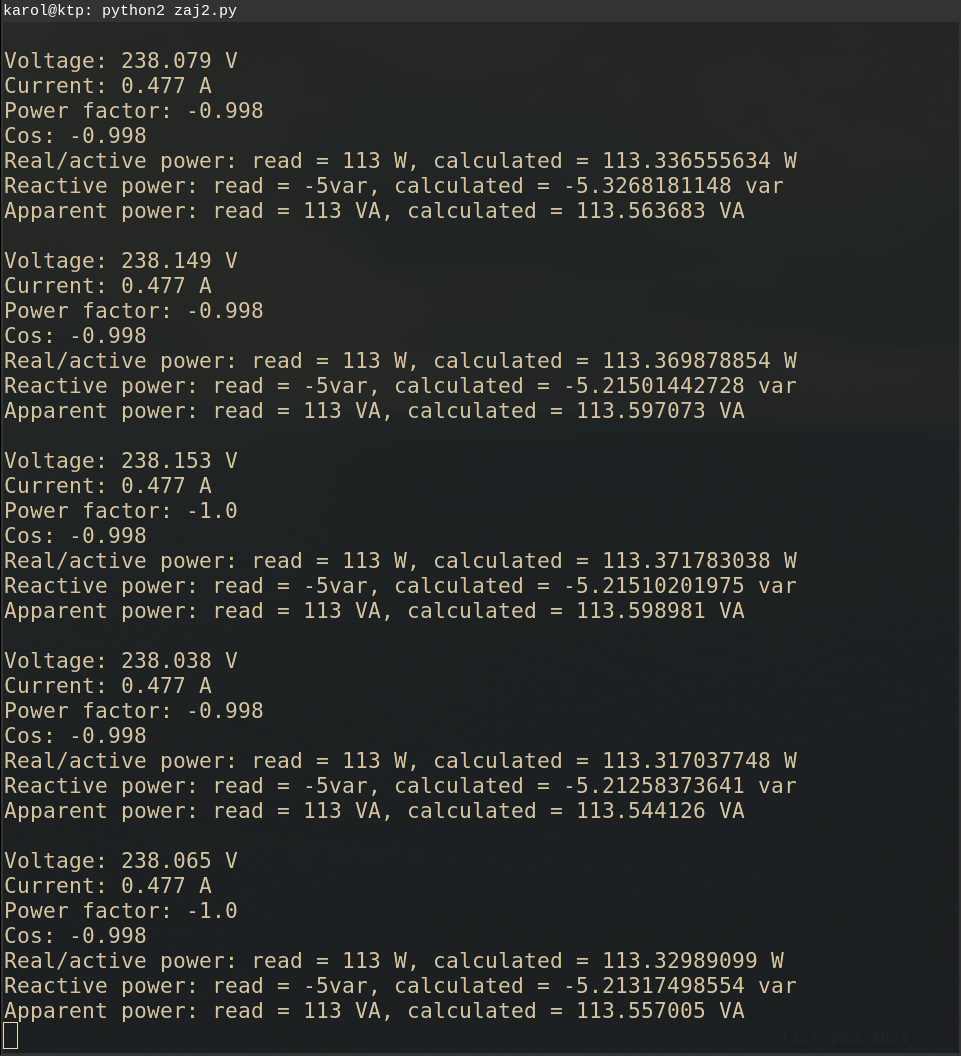
\includegraphics{zaj2lamp.png}
	   }
	\end{figure}
\end{minipage}
\begin{minipage}[c]{0.49\linewidth}
	\begin{figure}[H]
	   \centering
	   \resizebox*{\textwidth}{!}{
		  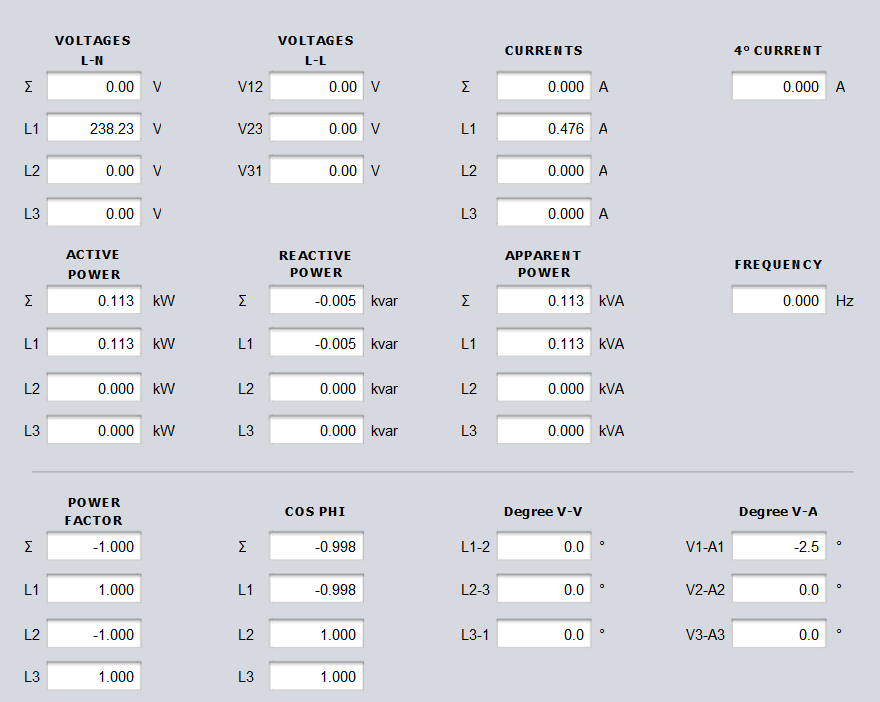
\includegraphics{app2lamp.png}
	   }
	\end{figure}
\end{minipage}
\begin{center}
	pomiary laptopa
\end{center}
\begin{minipage}[c]{0.49\linewidth}
	\begin{figure}[H]
	   \centering
	   \resizebox*{\textwidth}{!}{
		  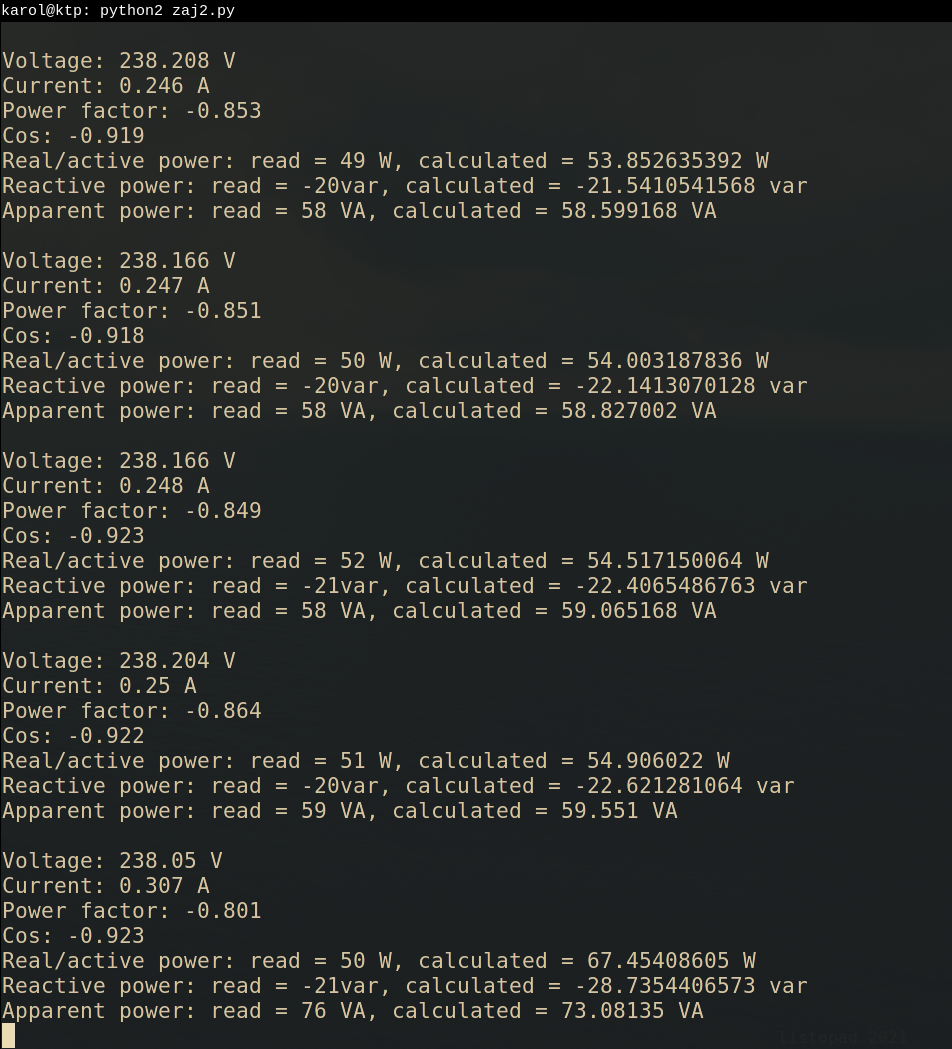
\includegraphics{zaj2.png}
	   }
	\end{figure}
\end{minipage}
\begin{minipage}[c]{0.49\linewidth}
	\begin{figure}[H]
	   \centering
	   \resizebox*{\textwidth}{!}{
		  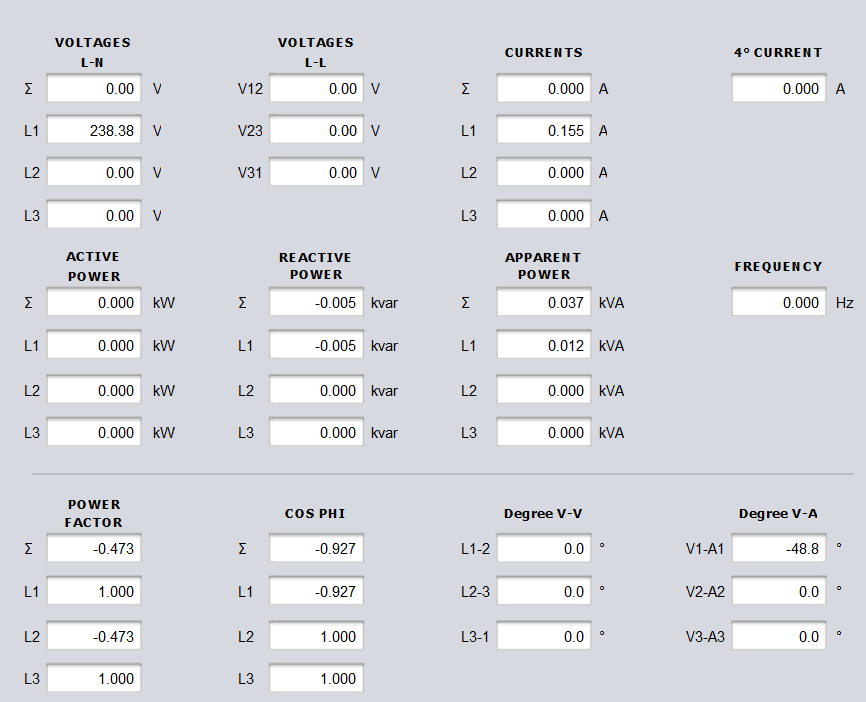
\includegraphics{app2laptop.png}
	   }
	\end{figure}
\end{minipage}\\

Zadania były w miarę proste, wszystkie udało się nam wykonać po przeczytaniu dokumentacji, kod napisaliśmy w pythonie z wykorzystaniem biblioteki pyModbusTCP.
Problemy na który się natknęliśmy to:
\begin{itemize}
	\item W aplikacji pola "Power Factor", dokładnie to L1 oraz L2 były zamienione.
	\item błędy gdy do urządzenia była podłączona więcej niż jedna aplikacja.
\end{itemize}


% \section{Pomocne materiały}
% \href{https://www.codeproject.com/articles/20929/simple-modbus-protocol-in-c-net-2-0}{Kod c# z modbus}
\end{document}